%% Nothing to modify here.
%% make sure to include this before anything else

\documentclass[10pt]{beamer}

% packages
\usepackage{color}
\usepackage{listings}
\usepackage{graphicx}
\usepackage{array}

% color definitions
\definecolor{mygreen}{rgb}{0,0.6,0}
\definecolor{mygray}{rgb}{0.5,0.5,0.5}
\definecolor{mymauve}{rgb}{0.58,0,0.82}
\definecolor{php-blue}{HTML}{8892BF}

\setbeamercolor{progress bar}{fg=php-blue}
\setbeamercolor{frametitle}{bg=php-blue}
\setbeamercolor{title separator}{fg=php-blue}
\setbeamercolor{progress bar in section page}{fg=php-blue}
\setbeamercolor{progress bar in head/foot}{fg=php-blue}

% preset-listing options
\lstset{
  backgroundcolor=\color{white},
  % choose the background color;
  % you must add \usepackage{color} or \usepackage{xcolor}
  basicstyle=\footnotesize,
  % the size of the fonts that are used for the code
  breakatwhitespace=false,
  % sets if automatic breaks should only happen at whitespace
  breaklines=true,                 % sets automatic line breaking
  captionpos=b,                    % sets the caption-position to bottom
  commentstyle=\color{mygreen},    % comment style
  % deletekeywords={...},
  % if you want to delete keywords from the given language
  extendedchars=true,
  % lets you use non-ASCII characters;
  % for 8-bits encodings only, does not work with UTF-8
  frame=single,                    % adds a frame around the code
  keepspaces=true,
  % keeps spaces in text,
  % useful for keeping indentation of code
  % (possibly needs columns=flexible)
  keywordstyle=\color{blue},       % keyword style
  % morekeywords={*,...},
  % if you want to add more keywords to the set
  numbers=left,
  % where to put the line-numbers; possible values are (none, left, right)
  numbersep=5pt,
  % how far the line-numbers are from the code
  numberstyle=\tiny\color{mygray},
  % the style that is used for the line-numbers
  rulecolor=\color{black},
  % if not set, the frame-color may be changed on line-breaks
  % within not-black text (e.g. comments (green here))
  stepnumber=1,
  % the step between two line-numbers.
  % If it's 1, each line will be numbered
  stringstyle=\color{mymauve},     % string literal style
  tabsize=4,                       % sets default tabsize to 4 spaces
  title=\lstname
  % show the filename of files included with \lstinputlisting;
  % also try caption instead of title
}

% macro for code inclusion
\newcommand{\includecode}[2][c]{
	\lstinputlisting[caption=#2, style=custom#1]{#2}
}

\usepackage[english]{babel}
% \usepackage[ngerman]{babel}

\usepackage[utf8]{inputenc}
\usetheme{metropolis}

\newcommand{\course}{
	PHP-Kurs
}

\author{
	Alexander Lichter
}

\lstset{
	language = PHP,
	showspaces = false,
	showtabs = false,
	showstringspaces = false
}

% meta-information
\newcommand{\topic}{
	% TODO fill in the actual topic
	PHP-Einführung
}

\title{\topic}
\date{\today}

% the actual document
\begin{document}

\maketitle

\begin{frame}{What's up today?}
	\setbeamertemplate{section in toc}[sections numbered]
	\tableofcontents
\end{frame}

\section{Before we dive in}

\begin{frame}{Before we dive in}

	Before we start, some questions for you:
	\pause
	\begin{itemize}
        \item What do you expect from the course? 	\pause
		\item Do you already have knowledge in programming?
	\end{itemize}
\end{frame}


\section{Requirements and stuff}

\begin{frame}{Requirements and stuff}
	Requirements

	\begin{itemize}
        \item A computer (obviously) 	\pause
		\item A decent OS 	\pause
		\item Knowledge in other programming languages will help 	\pause
	\end{itemize}
	Proceeding

	\begin{itemize}
		\item There will be 14 lessons
		\item Each covers a topic and comes with excercises
	\end{itemize}
\end{frame}

\section{Resources}
\begin{frame}{Some resources}
	\begin{itemize}
		\item You can ask your tutor (That's me :P)
		\item Join the Auditorium group \hfill \\
			\url{http://auditorium.inf.tu-dresden.de}
		\item StackOverflow \hfill \\
		\item Official documentation on \url{php.net/manual/} \pause
        \item Mailinglist \url{programmierung@ifsr.de}
        \item Cyberspace (wednesday 5./6. DS)
		\item Material-Repository \\
			\url{https://github.com/fsr/php-lessons}
	\end{itemize}
\end{frame}

\section{What is PHP}
\begin{frame}{PHP.. what?}
	PHP...
	\begin{itemize}
		\item ...is a recursive acronym for PHP: Hypertext Preprocessor \pause
		\item ...is a server-side language \pause
		\item ...is widely-used \pause
		\item ...is open source \pause
		\item ...is a dynamic language \pause
		\item ...isn't as strict as other languages like C/C++/Java
	\end{itemize}
\end{frame}

\section{Pros and Cons}
\begin{frame}{Now to the Pros and Cons}
	Pros
	\begin{itemize}
		\item No need to compile \pause
		\item No types must be set \pause
		\item OOP is supported, but not mandatory \pause
		\item Can be embedded in HTML code \pause
		\item Cheap to set up \pause
		\item Flexible in terms of Database \pause
	\end{itemize}

	Cons
	\begin{itemize}
		\item Can get really messy when not properly used \pause
		\item Partly bad language design \pause
		\item Can be tedious to use without a proper framework \pause
		\item Crap for developing Desktop applications (obviously) \pause
	\end{itemize}

	But anyway, it's my server-side language of choice, and also the choice of many other people. And I hope it'll be yours too!
\end{frame}

\section{Installation}
\begin{frame}{Installation \#{}1}
	Manually installing PHP is easy on every UNIX system (Linux, MacOS), but can be very annoying on Windows machine. \pause

	That's why we won't install a XAMP(P)-stack manually! \pause

	XAMP?\pause
	\begin{itemize}
		\item X = Letter for the OS (Can be L for Linux, M for macOS or W for Windows) \pause
		\item A for Apache (Server) \pause
		\item M for MySQL/MariaDB (Database) \pause
		\item P for PHP (obviously) \pause
		\item another P for Perl (sometimes) \pause
	\end{itemize}

	All contents can be swapped too (Apache for nginx, MySQL for Postgres, PHP for Python and so on..)
\end{frame}

\begin{frame}{Installation \#{}2}

	That's the reason why we will use \textbf{XAMPP} \pause
	\begin{figure}
  		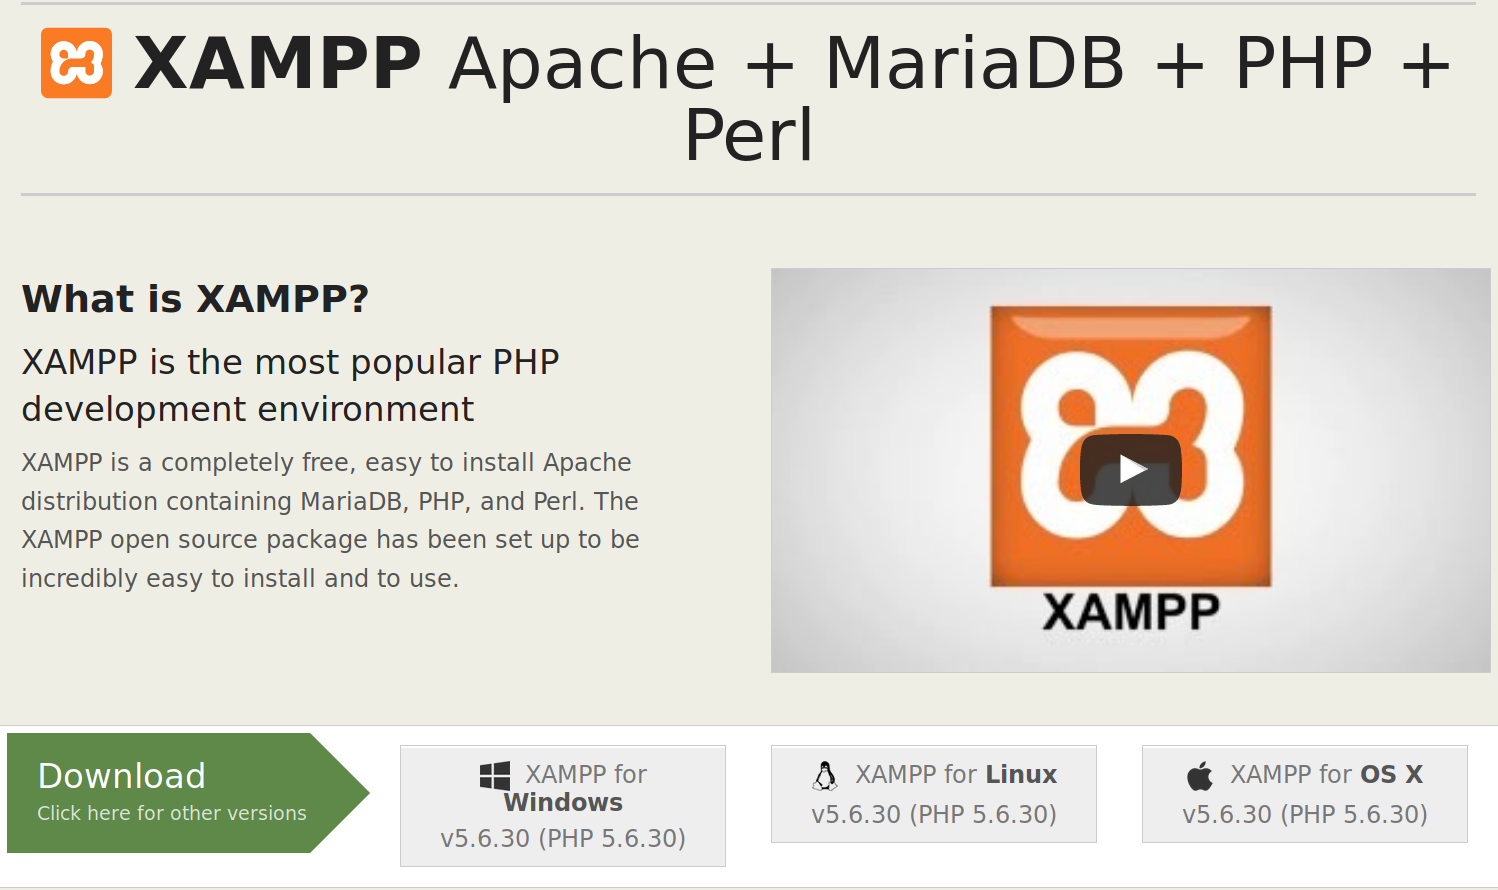
\includegraphics[width=\linewidth]{img/xampp.png}
	\end{figure}

	\pause

	Google \& install it! The instructions are very straightforward

\end{frame}

\begin{frame}{Installation \#{}3}

	Let's check if you did it right!

	If not already done, enable the Apache component in your XAMPP control panel. \pause

	Now navigate to \url{http://localhost} or \url{127.0.0.1}.

	In case you see a welcome screen, you did it right!

	\textbf{Any problems?} \pause

	Alright, let's continue

\end{frame}


\section{Programming Tools}

\begin{frame}{Programming Tools}

Now we setup our local environment, but there is one thing missing now.
With which program we will we write our code? \pause

	\begin{itemize}
		\item Word/LibreOffice \pause \textbf{NO!!!} \pause
		\item Terminal \pause \textbf{Possible, but tedious} \pause
		\item Notepad/Notepad++/Gedit \pause \textbf{Better.. but missing QoL\footnote{Quality of Life} features} \pause
		\item PHPStorm/Eclipse/... \pause \textbf{That's it!} \pause
	\end{itemize}

	We will use an IDE\footnote{Integrated Development Environment} later on!
	For our first little program we will go with Notepad++, TextMate or gedit, depending on your OS.

\end{frame}

\section{Let's get it on!}
\begin{frame}[fragile]{Here we go, our first program \#{}1}

For our first program, I will display the source code step by step here \pause

If not already done, enable your XAMPP (Apache should be enough) \pause

Change your directory to the "htdocs" directory of your XAMPP installation \pause

Create a new file called \textit{index.php} \pause

\end{frame}


\begin{frame}[fragile]{Here we go, our first program \#{}2}

Add the following code:

	\begin{lstlisting}
<?php

?>
	\end{lstlisting}

	\pause
	These are the PHP (open and close) tags. Whenever you write PHP code, you need to insert them before or after the code. \pause

	\emph{BEWARE:} It's a good practise to ommit the closing tag when you write PHP only (whenever you do not insert PHP inside an HTML file eg.). We will remove the closing tag from now on in those cases.
\end{frame}

\begin{frame}[fragile]{Here we go, our first program \#{}3}

After the opening tag our PHP code will be written. We are adding a \emph{Variable} here. Variables start with a dollar sign. \pause Now, we will assign the variable a value. In our case, it is your name. Words and senctences are called \emph{Strings} and are enclosed by single or double quotes.

	\begin{lstlisting}
<?php
	$name = "YOURNAMEHERE";

	\end{lstlisting}
\end{frame}

\begin{frame}[fragile]{Here we go, our first program \#{}2}

Now, we will print out a text with the name variable. Therefore we use \emph{echo}.
We could echo out a little text with the variable, like: \pause

	\begin{lstlisting}
<?php
	$name = "YOURNAMEHERE";
	echo "Welcome" . $name;
	\end{lstlisting}
	\pause



Let's open our file in the browser. Refresh the \url{http://localhost} page and you should see the text! \pause

Congrats! You wrote your first program.

\end{frame}


\section{Code style}
\begin{frame}[fragile]{Code Style - Some rules}

Before digging deeper into PHP stuff, a word on your (developing) code style\pause

\textbf{BE CONSISTENT!} \pause

There are several ways to write (semantically equivalent) code. Find your style, and stick with it!\pause

\textbf{INDENTS AND SPACES!} \pause

Please don't forget to indent code in function blocks or methods (more about this later) and to add proper spaces, for example when assigning variables. \pause


\textbf{SPEAKING IDENTIFIERS!} \pause

Name your variables properly. "\$a", "\$foo" or "\$test1" say nothing about the content, while "\$name", "\$codeStyleConfigItem" or "\$wellKnownParameterThatIsUsedEverywhere" likely give hints on what the variables are used\pause
\end{frame}


\begin{frame}[fragile]{Code Style - Examples}

A simple example:

\begin{lstlisting}
<?php
	$name = "YOURNAMEHERE"; //Readable, Speaking Identifiers and proper spacing
	$a='AnotherName'; // :(
	\end{lstlisting}

\end{frame}

\begin{frame}[fragile]{The end of the first part}

Hope you enjoyed our first lesson! \textbf{Any questions left?} \pause

See you next week!

\end{frame}




\end{document}
